\documentclass{article}

\usepackage[utf8]{inputenc}
\usepackage[T1]{fontenc}
\usepackage[portuguese]{babel}
\usepackage{amsmath, amsthm, amssymb}
\usepackage{graphicx}
\usepackage{bbm}

\author{Esdras R. Carmo - 170656}
\title{Aula PED de Integrais Duplas}
\date{\today}

% Comando para integral dupla sobre região R
\newcommand{\doubleint}[1] {\iint\limits_R #1 dA}

% Definição para os exemplos
\theoremstyle{definition}
\newtheorem{example}{Exemplo}[section]

\begin{document}
    \maketitle

    \section{Exercício 12, c)}
        Calcule:

        \begin{align*}
            \int_0^{\frac{\pi}{2}}\int_0^{\frac{\pi}{2}} \sin{x} \cos{y} dy dx &= \int_0^{\frac{\pi}{2}}\int_0^{\frac{\pi}{2}} \sin{x} \cos{y} dx dy\\
            &= \int_0^{\frac{\pi}{2}} \cos{y} \left( \int_0^{\frac{\pi}{2}} \sin{x} dx \right) dy\\
            &= \int_0^{\frac{\pi}{2}} \cos{y} \left[ -\cos{x} \right]_0^{\frac{\pi}{2}} dy\\
            &= \int_0^{\frac{\pi}{2}} \cos{y} dy = 1\\
        \end{align*}

    \section{Exercício 17, d)}
        Calcule o volume de $\{(x, y, z) \in \mathbbm{R}^3 \mid 0 \leq x \leq 1, 0 \leq y \leq 1, x^2 + y^2 \leq z \leq 2 \}$.
        Note a figura~\ref{fig:paraboloide-plano} que representa o que queremos calcular:

        \begin{figure}[h!]
            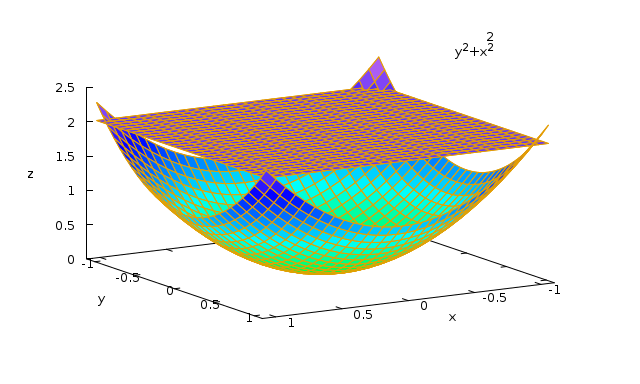
\includegraphics[width=\linewidth]{paraboloide-plano.png}
            \caption{Gráfico de $z$}
            \label{fig:paraboloide-plano}
        \end{figure}

        Assim temos:

        \begin{align*}
            V &= \int_0^1 \int_0^1 2 dx dy - \int_0^1 \int_0^1 (x^2 + y^2) dx dy\\
            V &= 2 - \int_0^1 \left[ \frac{x^3}{3} + y^2x \right]_0^1 dy\\
            V &= 2 - \left[ \frac{y^3}{3} + \frac{y}{3} \right]_0^1\\
            V &= 2 - \frac{2}{3} = \frac{4}{3}\\
        \end{align*}

    \section{Exercício 26}
        Calcule:

        \begin{align*}
            \int_0^1 \int_x^1 3y^4\cos{(xy^2)} dy dx
        \end{align*}

        Assim temos, $0 \leq y \leq 1$ e $0 \leq x \leq y$, representado em figura\ref{fig:retas-26}

        \begin{figure}[h!]
            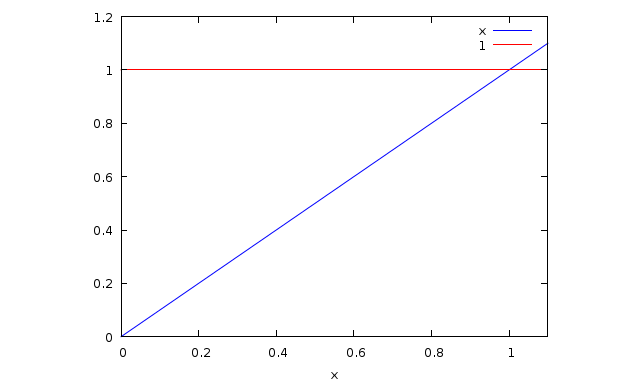
\includegraphics[width=\linewidth]{retas-26.png}
            \caption{Região de integração}
            \label{fig:retas-26}
        \end{figure}

        \paragraph{}
        Alterando a ordem de integração temos:

        \begin{align*}
            \int_0^1 \int_0^y 3y^4\cos{(xy^2)} dx dy &= \int_0^1 \left[ 3x^2 \sin{(xy^2)} \right]_0^y dy\\
            &= \int_0^1 [3y^2 \sin{y^3}] dy\\
            &= \int_0^1 (\sin{u}) du\\
            \int_0^1 \int_0^y 3y^4\cos{(xy^2)} dx dy &= [-\cos{u}]_0^1 = 1 - \cos{1}\\
        \end{align*}

    \section{Exercício 37}
        Considere a seguinte integral:

        \begin{align*}
            V &= \int_0^1 \int_0^y (x^2 + y^2) dx dy + \int_1^2 \int_0^{2 - y} (x^2 + y^2) dxdy
        \end{align*}
        
        \begin{enumerate}
            \item Esboce a região de integração:\\
                Veja Figura~\ref{fig:retas-37}
                \begin{figure}[h!]
                    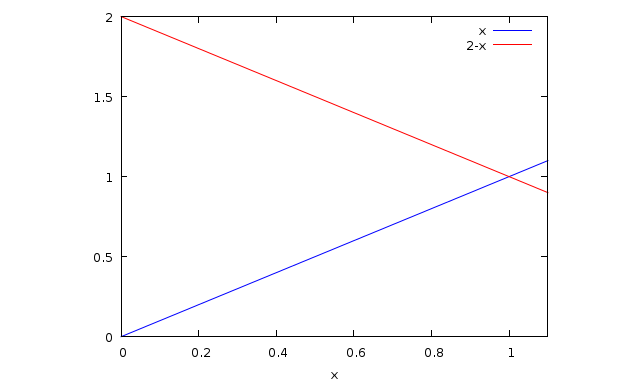
\includegraphics[width=\linewidth]{retas-37.png}
                    \caption{Região de integração}
                    \label{fig:retas-37}
                \end{figure}

            \item Mude a ordem de integração:
                \begin{align*}
                    V &= \int_0^1 \int_x^{2 - x} (x^2 + y^2) dy dx\\
                    R &= \{ (x, y) \in \mathbbm{R}^2 \mid 0 \leq x \leq 1, x \leq y \leq 2 -x \}
                \end{align*}

            \item Resolva a integral:
                \begin{align*}
                    \int_0^1 \int_x^{2 - x} (x^2 + y^2) dy dx &= \int_0^1 \left[ x^2y + \frac{y^3}{3} \right]_x^{2-x} dx\\
                    &= \int_0^1 \left[(2-x)x^2 + \frac{(2-x)^3}{3} - x^3 - \frac{x^3}{3} \right] dx = \frac{4}{3}\\
                \end{align*}

                A partir daí, a resolução fica a cargo do leitor.
        \end{enumerate}

    \section{Exercício 30 c)}
        Determine o volume do sólido abaixo de $z = xy$ e acima do triângulo de vértices $(1, 1)$, $(4, 1)$, $(1, 2)$.
        Dessa forma, temos o intervalo:

        \begin{align*}
            1 &\leq x \leq 4\\
            1 &\leq y \leq -\frac{1}{3}x + \frac{7}{3}\\
        \end{align*}

        Resolvendo a integral, temos:

        \begin{align*}
            V &= \int_1^4 \int_1^{\frac{7}{3} - \frac{1}{3}x} xy dy dx\\
            V &= \int_1^4 \left[ \frac{xy^2}{2} \right]_1^{\frac{7}{3} - \frac{1}{3}x} dx\\
            V &= \int_1^4 \frac{x}{2} \left[ \left( \frac{7}{3} - \frac{1}{3}x \right)^2 - 1 \right] dx\\
            V &= \left[ \frac{49x^2}{36} - \frac{14x^3}{54} + \frac{x^4}{72} - \frac{x^2}{4} \right]_1^4\\
        \end{align*}

        O restante fica a cargo do leitor.
\end{document}
